\documentclass[12pt]{scrartcl}
\usepackage[sexy]{james}
\usepackage[noend]{algpseudocode}
\setlength{\marginparwidth}{2cm}
\usepackage{answers}
\usepackage{array}
\usepackage{tikz}
\usepackage{graphicx}
\newenvironment{allintypewriter}{\ttfamily}{\par}
\usepackage{listings}
\usepackage{xcolor}
\usetikzlibrary{arrows.meta}
\usepackage{color}
\usepackage{mathtools}
\newcommand{\U}{\mathcal{U}}
\newcommand{\E}{\mathbb{E}}
\usetikzlibrary{arrows}
\Newassociation{hint}{hintitem}{all-hints}
\renewcommand{\solutionextension}{out}
\renewenvironment{hintitem}[1]{\item[\bfseries #1.]}{}
\renewcommand{\O}{\mathcal{O}}
\declaretheorem[style=thmbluebox,name={Chinese Remainder Theorem}]{CRT}
\renewcommand{\theCRT}{\Alph{CRT}}
\setlength\parindent{0pt}
\usepackage{sansmath}
\usepackage{pgfplots}

\usetikzlibrary{automata}
\usetikzlibrary{positioning}  %                 ...positioning nodes
\usetikzlibrary{arrows}       %                 ...customizing arrows
\newcommand{\eqdef}{=\vcentcolon}
\newcommand{\lint}{\int_{\overset{a}{\_}}^b}
\newcommand{\uint}{\int_a^{\bar{b}}}
\newcommand{\tr}{{\rm tr\ }}
\newcommand{\im}{{\rm Im\ }}
\newcommand{\spann}{{\rm span\ }}
\newcommand{\Col}{{\rm Col\ }}
\newcommand{\Row}{{\rm Row\ }}
\newcommand{\dint}{\displaystyle\int}
\newcommand{\dt}{\ {\rm d }t}
\newcommand{\PP}{\mathbb{P}}
\newcommand{\horizontal}{\par\noindent\rule{\textwidth}{0.4pt}}
\usepackage[top=3cm,left=3cm,right=3cm,bottom=3cm]{geometry}
\newcommand{\mref}[3][red]{\hypersetup{linkcolor=#1}\cref{#2}{#3}\hypersetup{linkcolor=blue}}%<<<changed

\tikzset{node distance=4.5cm, % Minimum distance between two nodes. Change if necessary.
         every state/.style={ % Sets the properties for each state
           semithick,
           fill=cyan!40},
         initial text={},     % No label on start arrow
         double distance=4pt, % Adjust appearance of accept states
         every edge/.style={  % Sets the properties for each transition
         draw,
           ->,>=stealth',     % Makes edges directed with bold arrowheads
           auto,
           semithick}}


% Start of document.
\newcommand{\sep}{\hspace*{.5em}}

\pgfplotsset{compat=1.18}
\begin{document}
\title{MATH410: Homework 9}
\author{James Zhang\thanks{Email: \mailto{jzhang72@terpmail.umd.edu}}}
\date{\today}

\definecolor{dkgreen}{rgb}{0,0.6,0}
\definecolor{gray}{rgb}{0.5,0.5,0.5}
\definecolor{mauve}{rgb}{0.58,0,0.82}

\lstset{frame=tb,
  language=Java,
  aboveskip=3mm,
  belowskip=3mm,
  showstringspaces=false,
  columns=flexible,
  basicstyle={\small\ttfamily},
  numbers=left,
  numberstyle=\tiny\color{gray},
  keywordstyle=\color{blue},
  commentstyle=\color{dkgreen},
  stringstyle=\color{mauve},
  breaklines=true,
  breakatwhitespace=true,
  tabsize=3
}

\maketitle

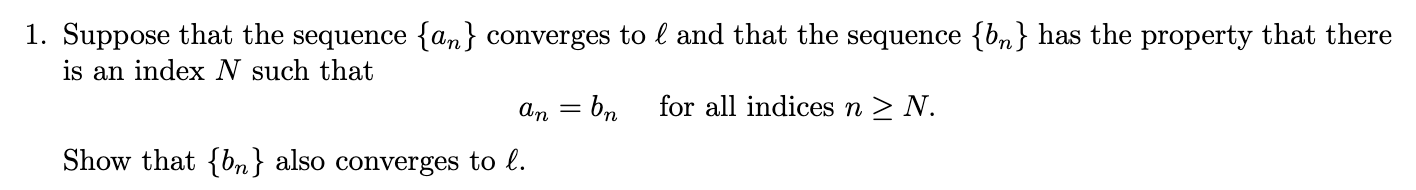
\includegraphics[width=14cm]{1.png}

\begin{proof}
  
\begin{enumerate}[a.]
  \item $\frac{d}{dx} \left( \int_0^x x^2 t^2 dt \right) = \frac{5x^4}{3}$
  
  $x^2t^2$ is a polynomial and so it is continuous. Note that $x^2$ is a constant respect to the integral. Thus,
  \[\frac{d}{dx}(\int_0^x x^2t^2 dt) = \frac{d}{dx}(x^2 * \int_0^x t^2 dt)\]
  By product rule and the Fundamental Theorem of Calculus 2, 
  \[= x^2(x^2) + 2x\int_0^x t^2 dt = x^4 + 2x\left(\frac{t^3}{3}\right)\Big|_0^x = x^4 + 2x(\frac{x^3}{3}) = x^4 + \frac{2x^4}{3} = \frac{5x^4}{3}\]
  \item $\frac{d}{dx}(\int_1^{e^x} \ln t dt) = xe^x$
  
  $\ln t$ is continuous on $[1, \infty)$. Using the Corollary following the Fundamental Theorem of Calculus 2 involving the Chain Rule, 
  \[\frac{d}{dx}(\int_1^{e^x} \ln t dt) = \ln(e^x) * e^x = xe^x\]
  \item $\frac{d}{dx}(\int_{-x}^x e^{t^2} dt) = $
  
  $e^{t^2}$ is continuous on $[-x, x]$. By additivity of integrals and derivatives, 
  \[\frac{d}{dx}(\int_{-x}^x e^{t^2} dt) = \frac{d}{dx}(\int_{-x}^0 e^{t^2} dt) + \frac{d}{dx}(\int_0^x e^{t^2} dt)\]
  \[= -\frac{d}{dx}(\int_0^{-x} e^{t^2} dt) + \frac{d}{dx}(\int_0^x e^{t^2} dt)\]
  Now we can use FTC2 and chain rule for the first term
  \[-e^{(-x)^2} * -1 + e^{x^2} = 2e^{x^2}\]
\end{enumerate}

\end{proof}

\newpage 

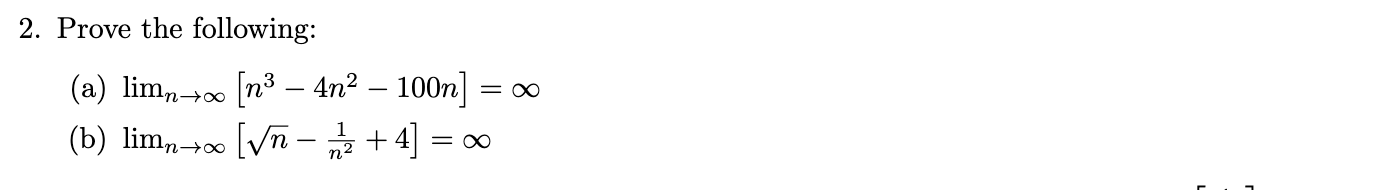
\includegraphics[width=14cm]{2.png}
\begin{proof}
  $f: \RR \to \RR$ being differentiable implies continuity. By additivity of integrals, 
  \[H'(x) = \frac{d}{dx}(\int_{-x}^0 (f(t) + f(-t)) + \int_0^x (f(t) + f(-t)) dt)\]
  By additivity of derivatives,
  \[H'(x) = \frac{d}{dx}(\int_{-x}^0 f(t) + f(-t) dt) + \frac{d}{dx}(\int_0^x f(t) + f(-t) dt)\]
  \[H'(x) = -\frac{d}{dx}(\int_0^{-x} f(t) + f(-t) dt) + \frac{d}{dx}(\int_0^x f(t) + f(-t) dt)\]
  \[H'(x) = f(-x) + f(x) + f(x) + f(-x) = 2f(x) + 2f(-x)\]
  by applying the Fundamental Theorem of Calculus 2. Now taking the second derivative, 
  \[H''(x) = 2f'(x) + 2f'(-x)\]
\end{proof}
\newpage 

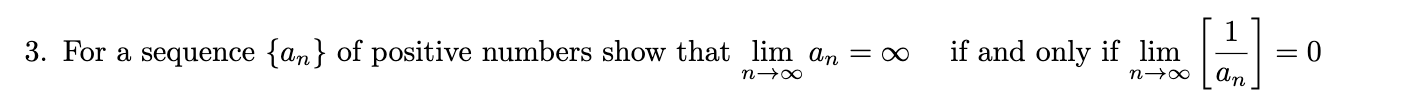
\includegraphics[width=14cm]{3.png}
\begin{proof}
    First, let's consider the integral term, and apply distributive property and additivity of integrals such that we obtain
    \[\int_0^x (x-t)f''(t) = \int_0^x xf''(t) dt - \int_0^x tf''(t) dt\]
    Observe that 
    \[\frac{d}{dx}(\int_0^x x f''(t) dt) = \frac{d}{dx}(x * \int_0^x f''(t) dt) = xf''(x) + \int_0^x f''(t) dt\]
    \[\frac{d}{dx}(\int_0^x t f''(t) dt) = xf''(x)\]
    which implies that $\frac{d}{dx}(\int_0^ x (x-t)f''(t) dt) = \int_0^x f''(t) dt$. By the Fundamental Theorem of Calculus 1, 
    \[\int_0^x f''(t) = f'(x) - f'(0)\]
    which implies that 
    \[\frac{d}{dx}(\int_0^x (x-t)f''(t) dt) = f'(x) - f'(0)\]
    Let $h, g: I \to \RR$ where $h(x) = f(x) - f'(0)x$, $g(x) = \int_0^x (x-t)f''(t)dt$, and $I = (-\infty, \infty)$. Observe that 
    \[g'(x) = f'(x) - f'(0) = h'(x)\]
    which by the Identity Criterion, shows that $h, g$ differ by a constant for all $c \in \RR \ \forall \ x$, or mathematically, 
    $h(x) = c + g(x) \ \forall \ x$. Since this is true for all $x$, let $x = 0 \implies f(0) - f'(0)(0) = c + \int_0^0 (0-t)f''(t) dt \implies c = f(0)$.
    Therefore, we conclude that 
    \[h(x) = f(0) + g(x) \ \forall \ x\] 
    \[f(x) - f'(0)x = f(0) + \int_0^x (x-t)f''(t) dt \ \forall \ x\]
    \[f(x) = f(0) + f'(0)x + \int_0^x (x-t)f''(t) dt \ \forall \ x\]
    as desired.
\end{proof}
\newpage 

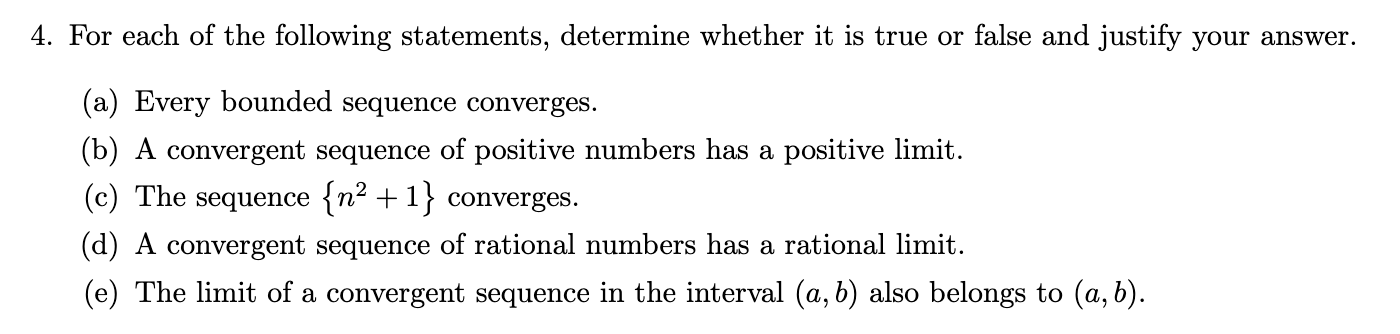
\includegraphics[width=14cm]{4.png}
\begin{proof}
  
  By additivity of derivatives, 
  \[\frac{d}{dx}\left[ F(x) - \int_a^x f\right] = \frac{d}{dx}(F(x)) -\frac{d}{dx}(\int_a^x f) = F'(x) - \frac{d}{dx}(\int_a^x f)\]
  By the given, which states that $F'(x) = f(x) \ \forall \ x \in (a,b)$. Note that $F(x) - \int_a^b f$ is continuous, since 
  both terms themselves are continuous so the difference is continuous. By the Fundamental Theorem of Calculus 2, 
  we get 
  \[\frac{d}{dx}\left[ F(x) - \int_a^x f\right] = f(x) - f(x) = 0 \ \forall \ x \in (a,b)\]
  as desired. Note that this is
  \[\frac{d}{dx}(F(x) - \int_a^x f) = 0 \implies f(x) = \frac{d}{dx}(\int_a^x f(t) dt) = \frac{d}{dx}(\int_a^x F'(t)dt)\]
  Now lets use this to construct a new proof for the First Fundamental Theorem, which states that
  if $F$ is continous on $[a,b]$ and differentiable on $(a,b)$ and $F': (a,b) \to \RR$ is continuous and bounded 
  then 
  \[\int_a^b F'(x) dx = F(b) - F(a)\]
  Let $g(x) = \int_a^x F'(t) dt$. Note that $g'(x) = F'(x)$. Therefore, $g$ and $F$ differ by a constant.
  \[g(x) = c + F(x)\]
  \[g(a) = \int_a^a F'(t) dt = 0 \implies g(a) = c + F(a) \implies c = -F(a)\]
  Therefore, 
  \[g(x) - F(x) = -F(a) \ \forall \ x \in [a,b]\]
  \[g(b) - F(b) = -F(a) \implies g(b) = F(b) - F(a) \implies \int_a^b F'(x) dx = F(b) - F(a)\]
  as desired.

\end{proof}
\newpage 

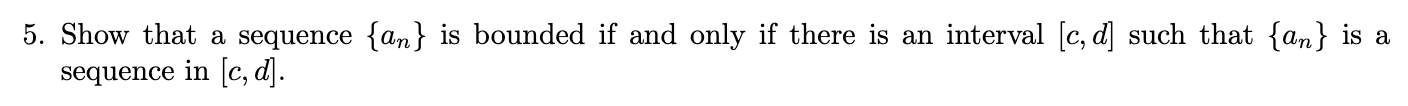
\includegraphics[width=14cm]{5.png}
\begin{proof}
  Recall that if $I$ is a neighborhood around $x_0$, then $f: I \to \RR$ and $g: I \to \RR$ 
  are said to have contact of order $n$ at $x_0$ if $f^{(k)}(x_0) = g^{(k)}(x_0) \ \forall \ k \in [0, n]$.
\hfill

\begin{enumerate}[a.]
  \item $f$ and $g$ have contact of order $1$ at $x_0$.
  \[k = 0 \implies f(0) = (0)^2 = 0 = \sin(0) = g(0)\]
   Note that
  \[f'(x) = 2x \implies f'(0) = 0\]
  \[g'(x) = \cos(x) \implies g'(0) = \cos(0) = 1\]
  Therefore, $g'(0) \neq f'(0)$ and so $f$ and $g$ have contact of order $0$ at $x_0 = 0$.

  \item $f$ and $g$ have contact of order $0$ at $x_0$
  \[k = 0 \implies f(0) = e^{0 * 0} = e^0 = 1, g(0) = 1 + 2(0)^2 = 1\]
  Now note that when $k = 1$
  \[f'(x) = 2xe^{x^2} \implies f'(0) = 0\]
  \[g'(x) = 4x \implies g'(0) = 0\]
  When $k = 2$, 
  \[f''(x) = (2x)(2xe^{x^2}) + 2e^{x^2} \implies f''(0) = 2\]
  by product rule.
  \[g''(x) = 4 \implies g''(0) = 4\]
  Therefore, $f$ and $g$ have contact of order $1$ at $x_0$.
\end{enumerate}

\end{proof}
\newpage 


\includegraphics[width=14cm]{6.png}
\begin{proof}
  Note that the sixth Taylor Polynomial of $f(x)$ is when $x_0 = 0$
  \[P_6(x) = \sum_{k=0}^6 \frac{f^{(k)}(0)}{k!}x^n \]
  \begin{align*}
    f(0) = 0 \\
    f'(x) = x^6e^x + 6x^5 e^x \implies f'(0) = 0\\
    f''(x) = x^6e^x + 6x^5e^x + 6x^5e^x + (6)(5)x^4 e^x \implies f''(0) = 0\\
    \vdots \\
    f^{(5)} \text{ has lowest term of degree 1 } \implies f^{(5)}(0) = 0\\
    f^{(6)}(x) = x^6e^x + \cdots + 6!e^x \implies f^{(6)}(0) = 6!
  \end{align*}
  Therefore, 
  \[P_n(6) = 0 + \cdots + 0 + \frac{6!}{6!}x^6 = x^6\]
\end{proof}
\newpage 

\includegraphics[width=14cm]{7.png}
\begin{proof}
  Let $f: (0, \infty) \to \RR$ such that $f(x) = (1 + x)^{1/3}$, and note that it is continuous and differentiable 
  because it is a rational function and $1 + x \neq 0 \ \forall \ x > 0$. Observe the following derivatives 
  \begin{align*}
    f'(x) = \frac{1}{3}(1 + x)^{-2/3} \\
    f''(x) = -\frac{2}{9}(1 + x)^{-5/3}\\ 
    f'''(x) = \frac{10}{27}(1 + x)^{-8/3}
  \end{align*}
  Consider the Taylor Polynomial expansion of $f(x)$ at $x_0 = 0$ 
  \[P_2(x) = f(0) + f'(0)x + \frac{f''(0)}{2!}x^2 = 1 + \frac{1}{3}x - \frac{1}{9}x^2\]
  Furthermore, consider the Lagrange Remainder where for each $x \neq 0, \ \exists c \in (0, x)$ such that  
  \[R_2(x) = \frac{f^{(3)}(c)}{3!}x^3 = \frac{5}{81}\frac{x^3}{(1+c)^{8/3}}\]
  Note that by the Lagrange Remainder Theorem that 
  \[f(x) = P_2(x) + R_2(x)\]
  However, $R_2(x) > 0$ because $x > 0, c > 0$. Therefore, $f(x) = P_2(x) + R_2(x) > P_2(x) \implies P_2(x) < f(x)$
  yields 
  \[1 + \frac{x}{3} - \frac{x^2}{9} < (1 + x)^{1/3} \ \ \ \ \ \ \ \ \ \ (*)\]
  Now for the other side of the inequality, consider
  \[R_1(x) = \frac{f''(c)}{2!}x^2 = -\frac{1}{9}\frac{x^2}{(1+x)^{5/3}} \implies R_1(x) < 0\]
  Therefore, $f(x) = P_1(x) + R_1(x) \implies f(x) < P_1(x)$
  \[ \implies (1 + x)^{1/3} < 1 + \frac{x}{3} \ \ \ \ \ \ \ \ \ \ (**)\]
  Combining $(*)$ and $(**)$, we obtain 
  \[1 + \frac{x}{3} - \frac{x^2}{9} < (1 + x)^{1/3} < 1 + \frac{x}{3}\]
  as desired.
\end{proof}

\end{document}

